\documentclass[a4paper]{article}

%% Language and font encodings
\usepackage[english]{babel}
\usepackage[utf8x]{inputenc}
\usepackage[T1]{fontenc}

%% Sets page size and margins
\usepackage[a4paper,top=3cm,bottom=2cm,left=3cm,right=3cm,marginparwidth=1.75cm]{geometry}
% keep figures in proper sections
\usepackage[section]{placeins}

%% Useful packages
\usepackage{bm}
\usepackage{amsmath}
\usepackage{graphicx}
\usepackage{listings}
\usepackage[colorinlistoftodos]{todonotes}
\usepackage[colorlinks=true, allcolors=blue]{hyperref}
\usepackage{booktabs}
\usepackage{longtable}
\usepackage{pgfplotstable}
\pgfplotsset{compat=1.9}% supress warning
\usepackage{array}
\newcolumntype{C}{>{\centering\arraybackslash}m{1.5cm}}
\newcolumntype{P}{>{\raggedright\arraybackslash}p{6.5cm}}

%% macros
\usepackage{mathtools}
\DeclarePairedDelimiter\abs{\lvert}{\rvert}%
\DeclarePairedDelimiter\norm{\lVert}{\rVert}%

\title{Modeling the Collective Forging Behavior of Ants on Uneven Terrain}
\author{You}

\begin{document}
\maketitle

\begin{abstract}
Ant foraging behavior is a collective decision making process in which, through individual interactions between ants and pheromone deposition, a colony of ants selects and exploits a path to follow between their nest and a food source. Research into the collective decision making strategies of ants, in addition to characterizing the biological mechanisms and emergent properties of the foraging process, has the potential to be leveraged into applications such as swarm robotics and commercial logistics management. Although ant foraging behavior has been extensively studied on flat terrains, ant foraging over uneven terrains is not well studied. This research presents an individual-based set of differential equations to model ant foraging behavior over uneven terrain in an enclosed arena. This model is employed to investigate the characteristics of foraging paths that ants tend towards when foraging over simple inclines of varying magnitudes. Numerical solutions of the model predict that, over most inclines, ants tend to favor the direct path between nest and food.
\end{abstract}

\section{Introduction}

Ant colonies regulate their foraging behavior through a collective decision making process; when ants forage, no individual ant operates with complete information about the terrain they are exploring. This contrasts with traditional human approaches decision-making, which typically centralize information, process it, then redistribute instructions. Consider, for example, traffic-aware navigation tools such as Waze or Google Maps; the distribution of traffic distribution across a geographic region is collected from users, centrally processed, and then routing instructions are redistributed to individual users. In contrast, collective intelligence on the level of the ant colony emerges from parallel execution of a simple set of individual pheromone deposit and response behaviors; among other feats, foraging ants will tend to choose the shortest path between nest and food and to selectively exploit the richest of an array of food sources.

My task was to extend mathematical models of ant foraging, which are well-developed on flat surfaces, to uneven terrains. It is well known that, as a collective, ants can optimize the foraging path they travel between nest and food. On flat terrain, a clear ``best'' path exists: the shortest-distance foraging path, the most energy-efficient path, and the quickest-trip path are all identical. On uneven terrains, however, this is no longer necessarily the case and the question of which trade-offs ants make -- and how they make them -- is of great interest. After surveying existing models of ant foraging behavior on flat terrain and individual ant behavior on inclined surfaces, I designed and numerically evaluated a differential equations-based model of the foraging behavior of ants over uneven terrain.

My model will see continued use, enabling the Swarm Lab to work out the rules by which real ants act on uneven terrain in a foraging context by simulating hypothesized behaviors and assessing the resulting foraging path predictions in comparison with upcoming in vivo ant foraging experiments. Ultimately, research into the collective intelligence of insects translates directly to technological applications; for example, such research has been leveraged in swarm robotics projects, such as NASA's ant-inspired ``Swarmies'' that may one day harvest resources for Martian colonies and distributed traffic management schemes (especially in relation to autonomous vehicles).

\section{Model}

\subsection{Experimental Design}
\begin{figure}[h]
    	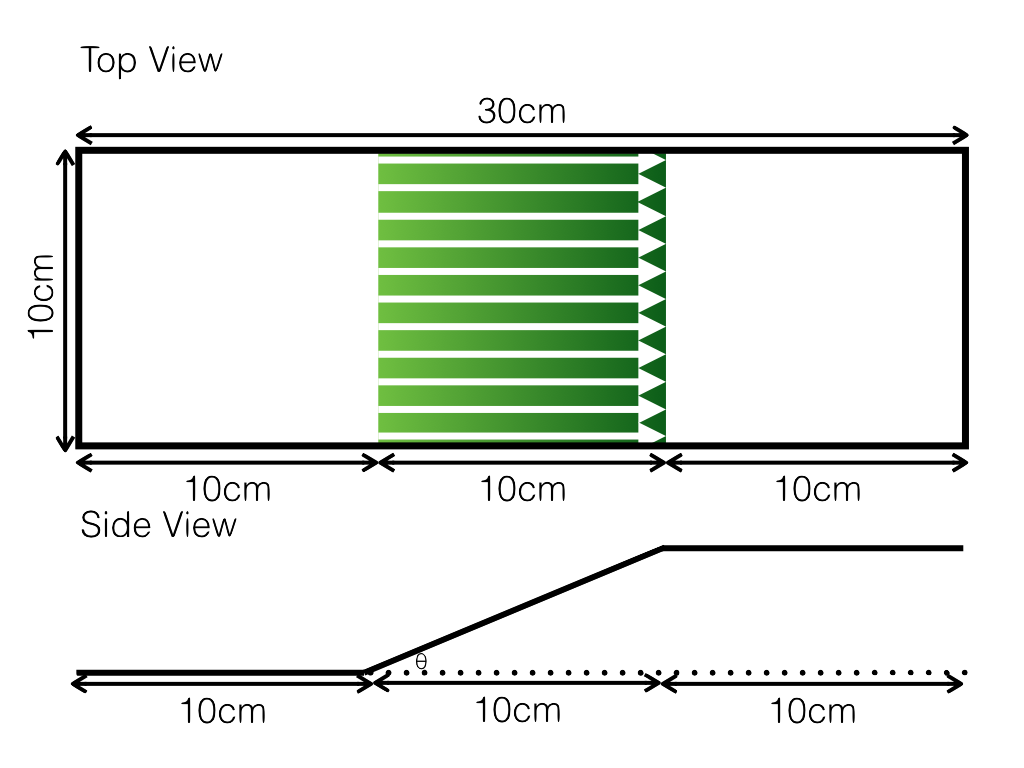
\includegraphics[width=0.4\textwidth]{img/model_components_cartoons_011}
      \caption{Arena terrain scheme}
\end{figure}






\begin{figure}[h]
    	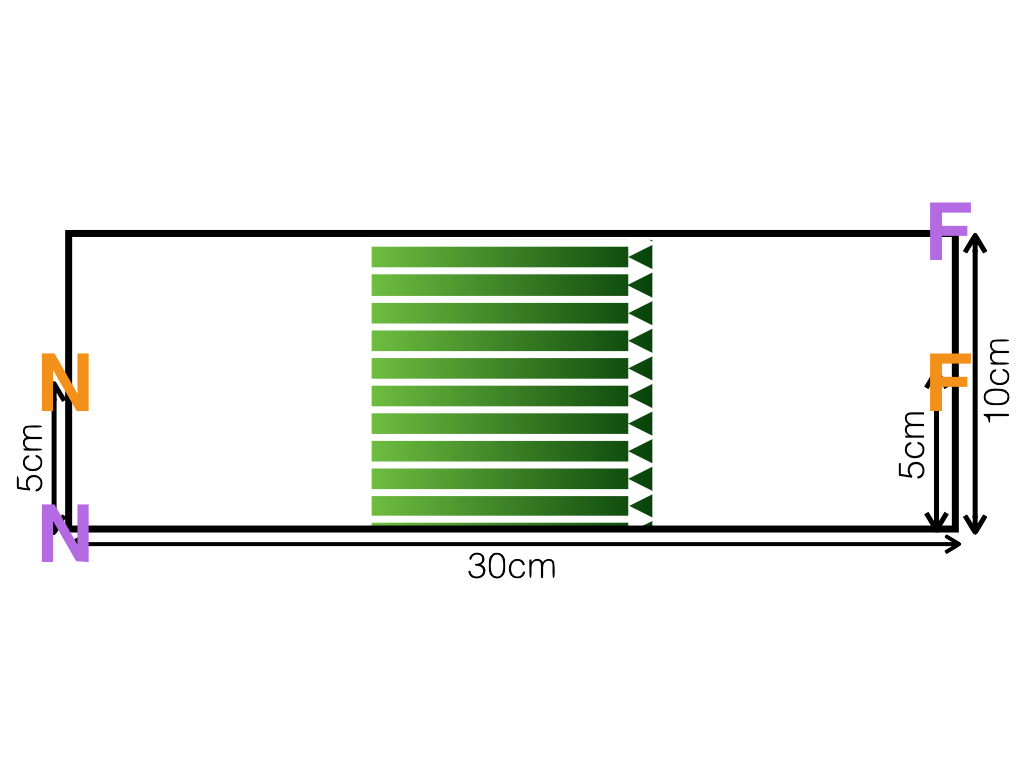
\includegraphics[width=0.4\textwidth]{img/model_components_cartoons_010}
				\vspace{-8ex}
				\caption{Nest and food placement scheme}
\end{figure}


\subsection{Modeling Considerations}

The model should consider:
	\begin{itemize}
    	\item self-propulsion,
        \item containment in arena,
        \item forager/returner roles (attraction to food, attraction to nest),
        \item random reorientation events (``Boltzmann walker''),
        \item physical effects of gravity on inclined terrain,
        \item behavioral phenomena on inclined terrain,
        \item pheromone deposit, and
        \item pheromone response behavior.
    \end{itemize}


\subsection{Random Reorientation Events (''Boltzmann Walker'')}
\begin{figure}[h]	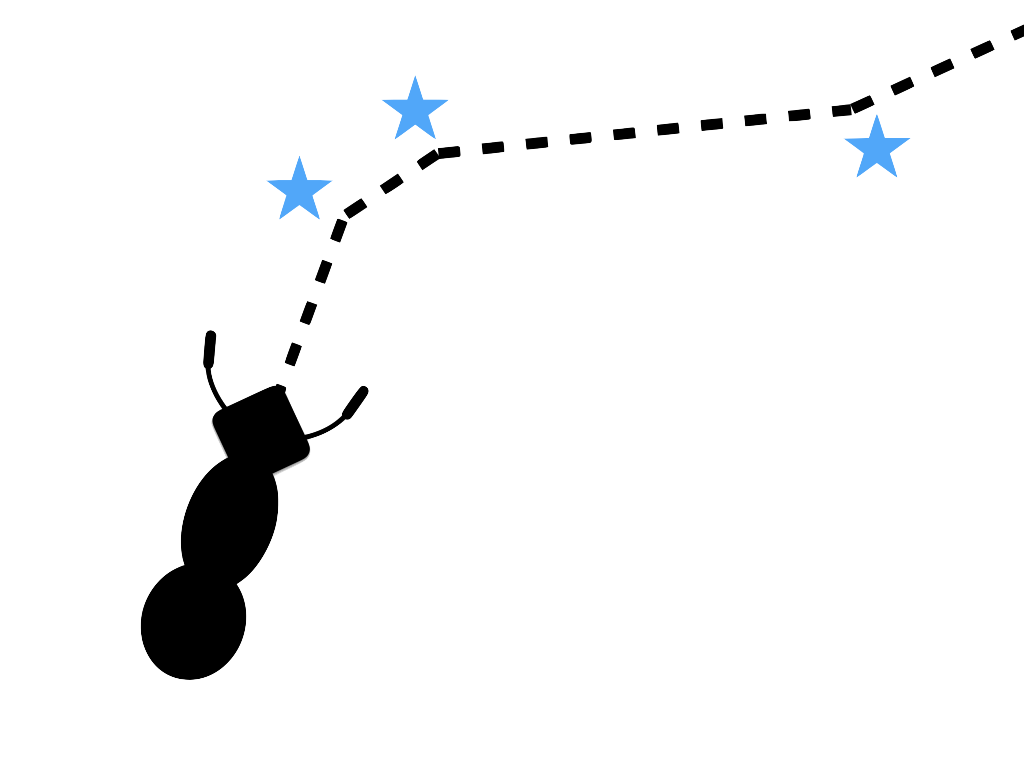
\includegraphics[width=0.4\textwidth]{img/model_components_cartoons_009}
		\caption{\footnotesize{``Boltzmann walker'' cartoon; blue stars denote random reorientation events.}}
\end{figure}
\begin{align*}
\frac{d}{dt} \begin{pmatrix}\vec{x}\\\vec{v}\\s\end{pmatrix} = \begin{pmatrix}\ldots \\ \ldots\\ \norm{v}\end{pmatrix}
\end{align*}
\begin{align*}
\theta_{\operatorname{new}} = \theta_{\operatorname{old}} + \bm{T} \\
s = 0 \\
s_{\operatorname{thresh}} = \bm{X}
\end{align*}


\begin{itemize}
		\item ant ``keeps track'' of how far it has traveled, $s$
    \item upon reaching a threshold distance ($s > s_{\operatorname{thresh}}$), the ant experiences a ``reorientation event''
    \item the threshold distance is generated from an exponential distribution ($\bm{X} \sim \mathit{exp}(\omega)$)
    \item ``memoryless property'' (probability of reorientation is uniform over every unit of distance the ant traverses)
    \item the angle the ant turns through is normally distributed  ($\Delta \theta = \bm{T} \sim \mathcal{N}(0,\sigma^2)$)
\end{itemize}

\subsection{Random Reorientation Events (``Boltzmann Walker'')}
\begin{align*}
\bm{T}_{\operatorname{effective}} = \bm{T} / \beta \\
\beta =
\begin{cases}
      \text{forager role} & e^{c_1p} \\
      \text{returner role} & c_2
\end{cases} \\
s_{\operatorname{thresh}} = \bm{X} + c_3 \frac{|\vec{s} \cdot \vec{v}|}{\norm{\vec{v}}}
\end{align*}

\begin{itemize}
  \item free path of ant ($s_{\operatorname{thresh}}$) increases if ant oriented with the gradient {\scriptsize\cite{khuong_how_2013}}
	\item severity of random reorientation should decrease with
    \begin{itemize}
    	\item pheromone detection (``following trail'')
      \item returner status
    \end{itemize}
    \item $p$ is maximum pheromone level sensed by ant
\end{itemize}

\subsection{Behavioral Response to Incline}

\begin{figure}[h]
\begin{minipage}[]{0.3\textwidth}
    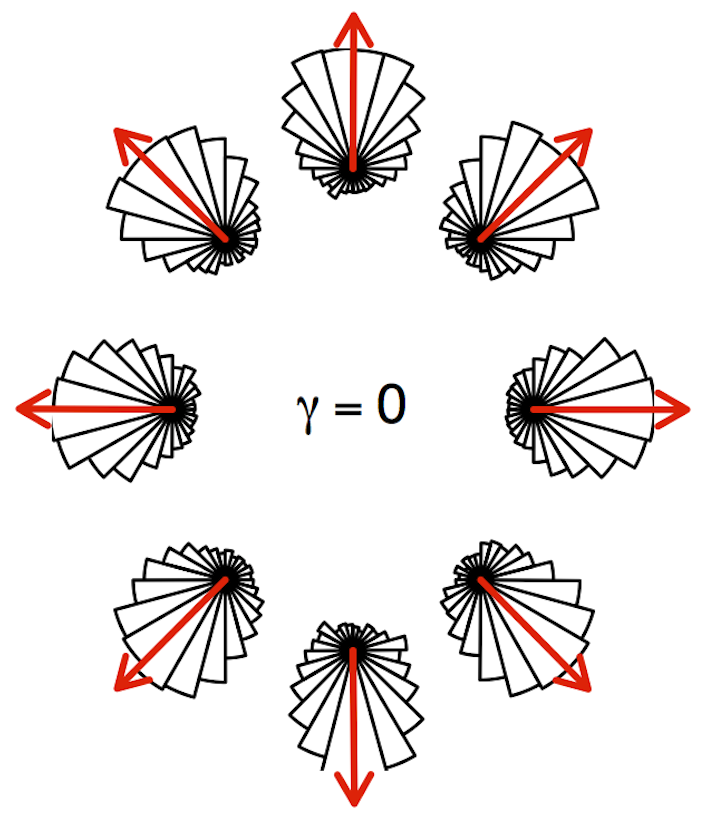
\includegraphics[width=\textwidth]{img/khuong_0}
\end{minipage}%
\begin{minipage}[]{0.05\textwidth}
~
\end{minipage}%
\begin{minipage}[]{0.3\textwidth}
    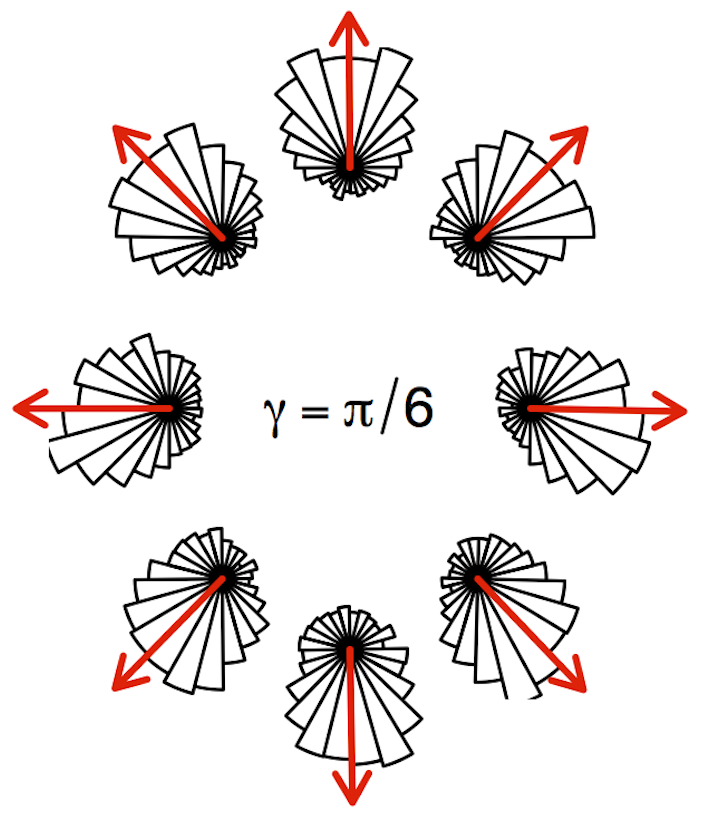
\includegraphics[width=\textwidth]{img/khuong_pi_div_6}
\end{minipage}%
\begin{minipage}[]{0.05\textwidth}
~
\end{minipage}%
\begin{minipage}[]{0.3\textwidth}
    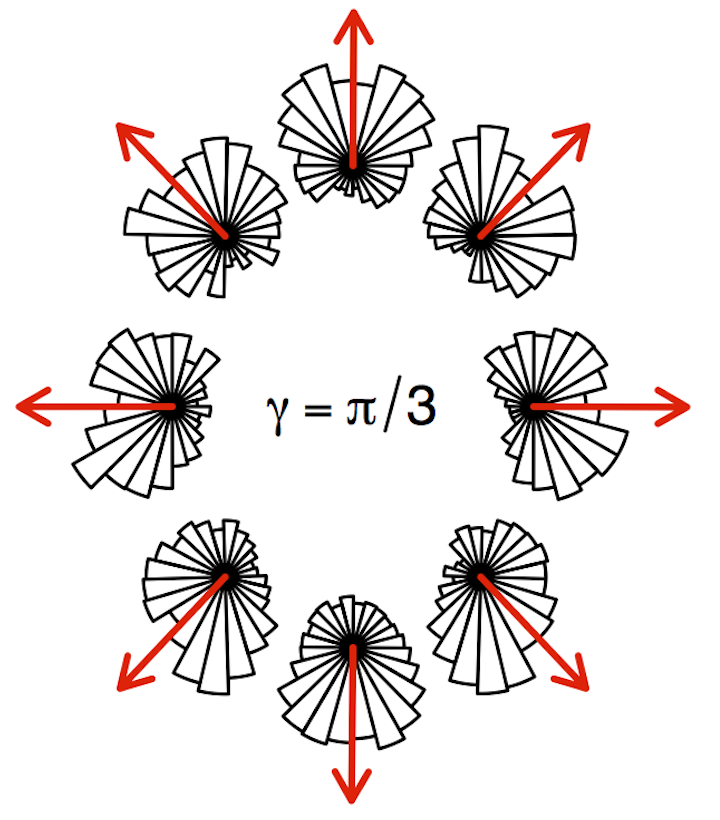
\includegraphics[width=\textwidth]{img/khuong_pi_div_3}
\end{minipage}%
\caption{Ant Reorientation on Inclined Surfaces \scriptsize{\cite{khuong_how_2013}}}
\end{figure}


\begin{itemize}
	\item ants preferentially re-orient themselves to align with or against a surface's topographical gradient {\cite{khuong_how_2013}}
    \item ants follow longer free paths when aligned with or against a surface's topographical gradient {\scriptsize\cite{khuong_how_2013}}
\end{itemize}


\subsection{Response to Pheromone}
\begin{align*}
\frac{d}{dt} \begin{pmatrix}\vec{x}\\\vec{v}\end{pmatrix} = \begin{pmatrix}\hdots\\ \hat{\vec{v}}_{\perp}(L - R)\end{pmatrix}
\end{align*}
\begin{itemize}
	\item ant integrates pheromone concentration over ``L'' and ``R'' quarter-circular regions
    \item ant accelerates perpendicular to its orientation
    \item magnitude of acceleration is proportional to the difference in concentration of pheromone over the ``L'' and ``R'' regions
\end{itemize}


\subsection{Self Propulsion}

\begin{align*}
			\frac{d}{dt} \begin{pmatrix}\vec{x}\\\vec{v}\end{pmatrix} = \begin{pmatrix}\vec{v}\\ \alpha \hat{\vec{v}}(\xi^2 - \norm{\vec{v}}^2)\end{pmatrix}
\end{align*}

\begin{itemize}
	\item ant accelerates in the direction of its movement if $\norm{\vec{v}}  \xi$
    \item ant accelerates against the direction of its movement if $\norm{\vec{v}} < \xi$
    \item``pushes'' ant towards a fixed speed
    \item $\alpha$ is a constant that governs the magnitude of this effect
\end{itemize}

\subsection{Attraction to Food/Nest}
\begin{align*}
\frac{d}{dt} \begin{pmatrix}\vec{x}\\\vec{v}\end{pmatrix} = \begin{pmatrix}\hdots \\ \beta_{\vec{x}} \frac{\vec{a} - \vec{x}}{\norm{\vec{a} - \vec{x}}} \end{pmatrix}
\end{align*}
\begin{itemize}
	\item ant experiences nest attraction if it is in the returner role
    \item ant experiences food attraction if it is in the forager role
	\item ant accelerates in the direction of the attractor
    \item if multiple attractors are present,
    \begin{itemize}
		\item ant is attracted to nearest food item
        \item ant is attracted to midpoint of nest items
    \end{itemize}
    \item $\beta_{\vec{x}}$ governs the strength of attraction
    \begin{itemize}
    	\item constant for nest attraction
        \item for food attraction, decays exponentially with distance from food
    \end{itemize}
\end{itemize}

\subsection{Near Nest Attraction}
\begin{align*}
\frac{d}{dt} \begin{pmatrix}\vec{x}\\\vec{v}\end{pmatrix} = \begin{pmatrix}
\hdots \\
\gamma_{\vec{x}} \hat{\vec{v}}_{\perp} \Big( \hat{\vec{v}}_{\perp} \cdot \frac{\vec{a} - \vec{x}}{\norm{\vec{a} - \vec{x}}} \Big)
\end{pmatrix}  \\
\beta = c_1e^{-c_2\norm{\vec{a} - \vec{x}}}
\end{align*}
\begin{itemize}
	\item ant experiences attraction with magnitude increasing exponentially with proximity to nest
    \item acceleration is projected onto vector perpendicular to orientation of ant
	\item ensures that ant goes directly to nest if ant is nearby the nest
\end{itemize}

\subsection{Pheromone Deposit}
\begin{align*}
\frac{d}{dt} p = \kappa f(p,s\vec{x}_1,\hdots,\vec{x}_n)
\end{align*}
\begin{itemize}
	\item the rate of pheromone deposit is proportional to total speed of ants located at a tile
    \item (ants only deposit pheromone when they move)
    \item let $f(p, \vec{x}_1,\hdots,\vec{x}_n)$ represent a sum of the speeds of of ants associated with the pheromone point $p$
    \item $\kappa$ is a constant governing the magnitude of pheromone deposit
\end{itemize}

\subsection{Complete Model}

\scriptsize
\centerline{
\begin{minipage}{\linewidth}
\begin{align*}
\frac{d}{dt}
\begin{pmatrix}
    \vec{x}_1 \\
    \vec{v}_1 \\
    s_1 \\
    \vdots \\
    p_1 \\
    \vdots
\end{pmatrix}
= \begin{pmatrix}
	\vec{v}_1 \\
    \alpha \hat{\vec{v}}_1 \Big[ \frac{c}{\norm{\vec{v}}} - a \norm{\vec{v}} + \frac{\norm{\vec{v}}^2 - b \vec{v} \cdot \nabla s}{\sqrt{\norm{\vec{v}}^2 + (\vec{v} \cdot \nabla s)^2}} \Big] + \beta_{\vec{x}} \frac{\vec{a} - \vec{x}_1}{\norm{\vec{a} - \vec{x}_1}} + \hat{\vec{v}}_{1\perp}(L_1 - R_1) + \gamma_{\vec{x}} \hat{\vec{v}}_{\perp} \Big( \hat{\vec{v}}_{\perp} \cdot \frac{\vec{a} - \vec{x}}{\norm{\vec{a} - \vec{x}}} \Big) \\
    \norm{\vec{v}_1} \\
    \vdots \\
    \kappa f(p_1, \vec{x}_1,\hdots,\vec{x}_n) + \lambda p_1 \\
    \vdots
\end{pmatrix}
\end{align*}
\end{minipage}
}
\normalsize
events:
\begin{itemize}
\item out of bounds $\rightarrow$ reflect heading to ``bounce'' ant
\item $s > s_{\operatorname{thresh}}$ $\rightarrow$ $s = 0$, $s_{\operatorname{thresh}} = \bm{X} + c_3 \frac{|\vec{s} \cdot \vec{v}|}{\norm{\vec{v}}}$, random reorientation event with gradient alignment bias
\item close to food/nest $\rightarrow$ switch forager/returner role
\end{itemize}

\subsection{Table of Parameters}
\noindent
\pgfplotstabletypeset[
    begin table=\begin{longtable},
    end table=\end{longtable}, 
    string type,
    col sep=comma,
    columns={name,value,unit,notes},
    columns/name/.style={column type=l},
    columns/value/.style={column type=c},
    columns/unit/.style={column type=c},
    columns/notes/.style={column type=P},
    every head row/.style={
        before row=\toprule,
        after row=
            \cmidrule(lr){1-1}
            \cmidrule(lr){2-2}
            \cmidrule(lr){3-3}
            \cmidrule(lr){4-4}
    },
    every last row/.style={after row=\bottomrule}
    ]{consts.csv}


\section{Results}

\subsection{Path Shape}
\FloatBarrier
\begin{figure}[!htb]
\begin{minipage}{0.33\textwidth}
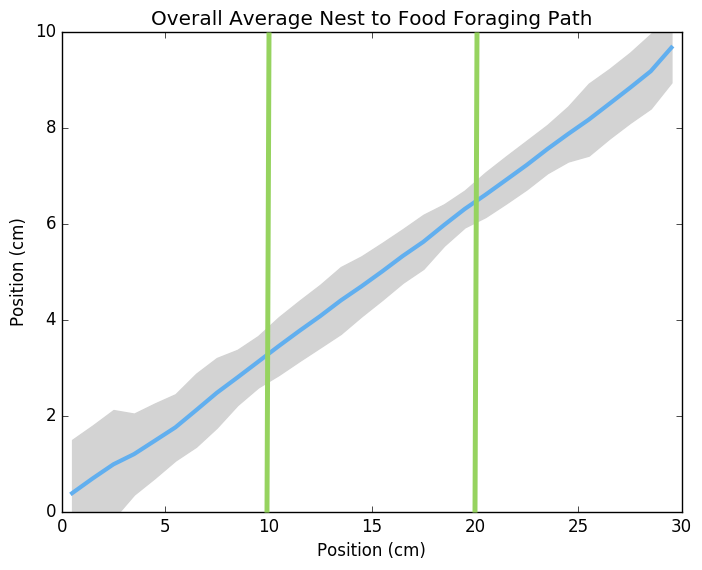
\includegraphics[width=\textwidth]{img/corner-to-corner-average_path_negpidiv3.png}
\end{minipage}%
\begin{minipage}{0.05\textwidth}
\end{minipage}%
\begin{minipage}{0.33\textwidth}
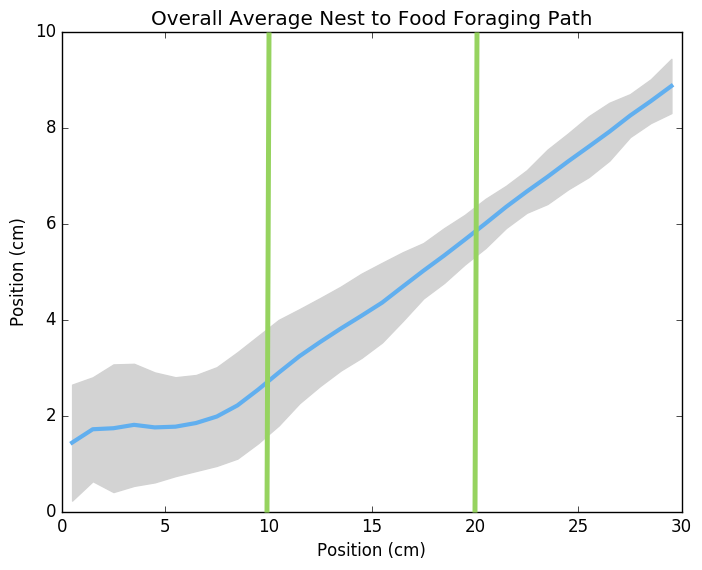
\includegraphics[width=\textwidth]{img/corner-to-corner-average_path_0.png}
\end{minipage}%
\begin{minipage}{0.05\textwidth}
\end{minipage}%
\begin{minipage}{0.33\textwidth}
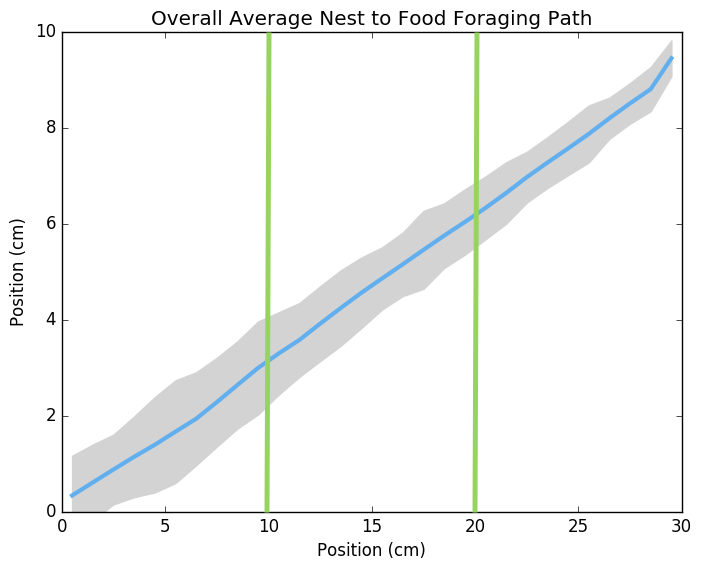
\includegraphics[width=\textwidth]{img/corner-to-corner-average_path_pidiv3.png}
\end{minipage}%

\caption{Comparison of overall average nest to food foraging path for, left to right, $-\pi/3$, $0$, and $\pi/3$ radian inclines.}
\end{figure}


\subsection{Path Length}
\FloatBarrier
\begin{figure}[!htb]
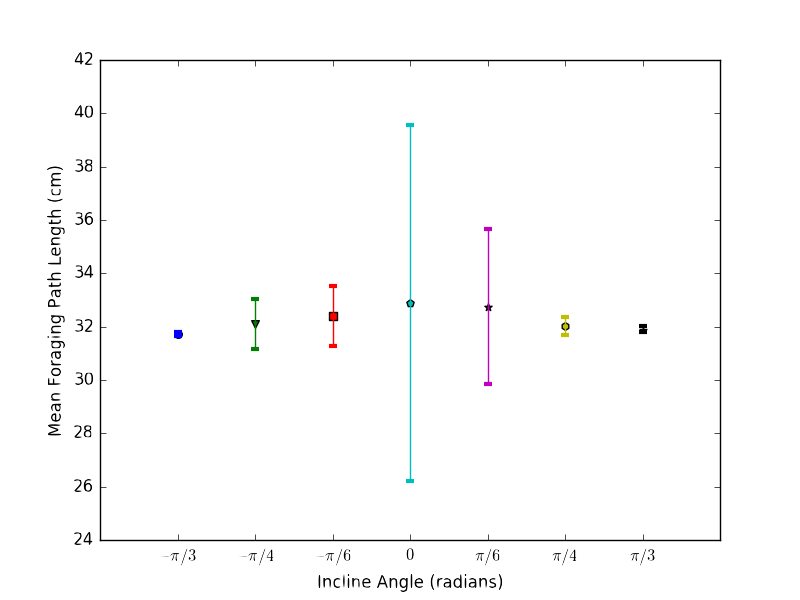
\includegraphics[width=0.4\textwidth]{img/corner-to-cornermeanforagingpathlength.png}
\caption{Comparison of path lengths over incline angles for corner-to-corner trials}
\end{figure}


\subsection{Trip Duration}
\FloatBarrier
\begin{figure}[!htb]
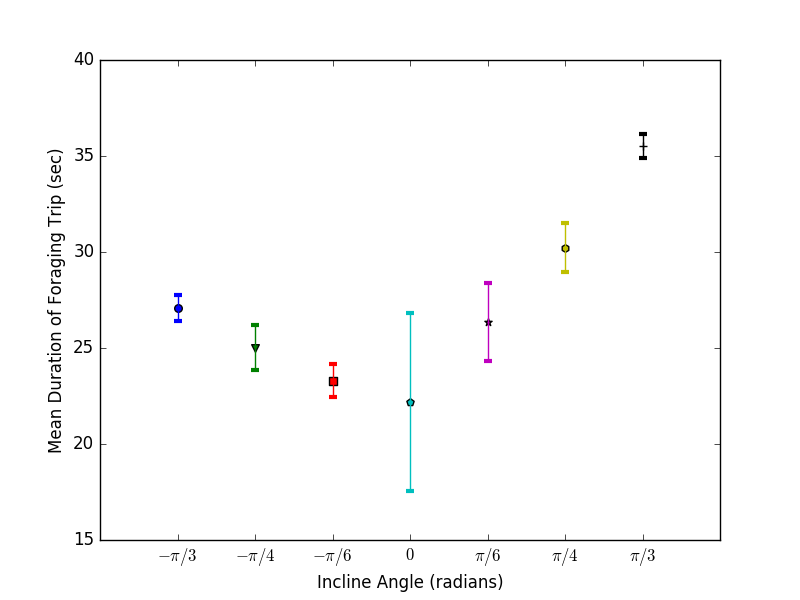
\includegraphics[width=0.4\textwidth]{img/corner-to-cornermeandurationofforagingtrip.png}
\caption{Comparison of trip durations over incline angles for corner-to-corner trials}
\end{figure}


\subsection{Summary}
\begin{itemize}
	\item as expected, foraging trips take longer over steeper incline and decline
	\begin{itemize}
		\item also taking longer over uphill versus downhill inclines
	\end{itemize}
	\vspace{1em}

	\item the foraging path is generally more stable with steep incline or decline
	\begin{itemize}
		%\item path is smoother
		\item ants are less likely to get lost/stuck
		\item this effect is less pronounced in the center-to-center arena
	\end{itemize}
	\vspace{1em}

	\item the foraging path becomes more direct with steeper incline or decline
	\vspace{-1em}
	\begin{itemize}
		\item even though the direct path is not aligned with the incline in the corner-to-corner arena
		\item this effect is less pronounced in the center-to-center arena
	\end{itemize}
\end{itemize}


\section{Discussion}

\subsection{Max Speed}
\begin{figure}[!htb]

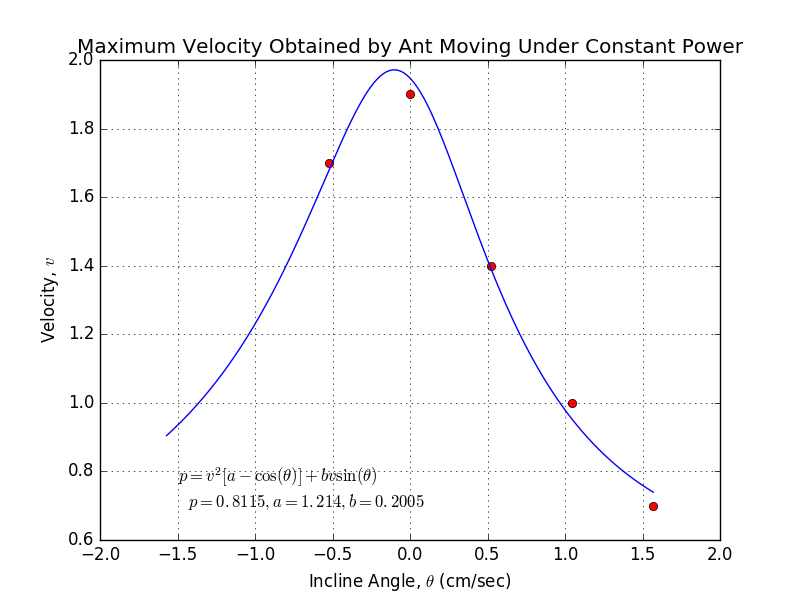
\includegraphics[width=0.4\textwidth]{img/const_power_velocity}

\end{figure}
\begin{align*}
 p = v^2(a - \cos(\theta)) + b \times v \times \sin(\theta) \\
  a = 1.214 \\
  b = 0.2005 \\
  p = 0.8115
\end{align*}


\subsection{Optimal Corner-to-Corner}
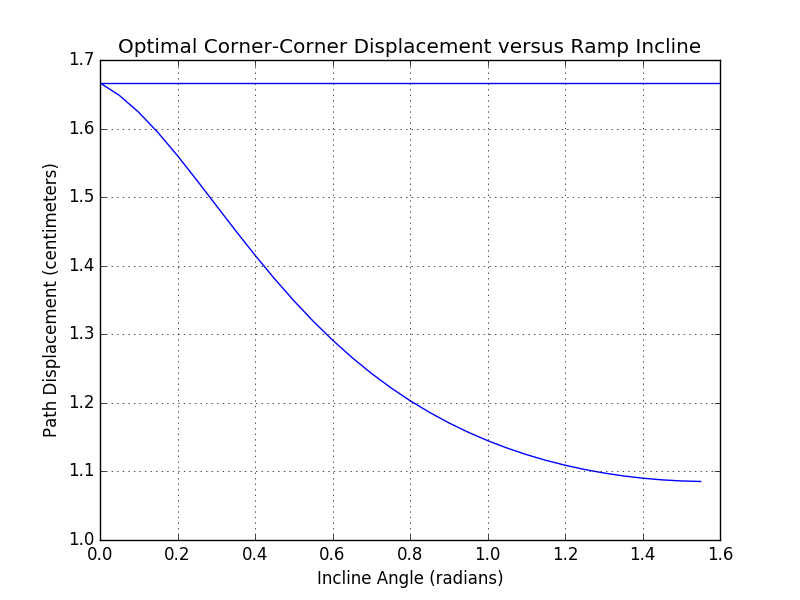
\includegraphics[width=0.5\textwidth]{img/optimal_corner_corner_displacement_versus_ramp_incline}
\begin{center}
\begin{tabular}{ c c c }
 incline & displacement (cm) & time (sec) \\ 
 0 & 1.6666666951743492 & 16.239124992741537 \\  
 math.pi/6 & 1.3347182872155725 & 18.030748007672663 \\
 math.pi/4 & 1.2086175733441706 & 18.955404943299744 \\
 math.pi/3 & 1.1347489653055225 & 19.589063308764256 \\
 math.pi/2 & 1.0852990219701015 & 20.06002493694109
\end{tabular} \\
\end{center}
displacement for a direct path: 1.666666666666667 cm

\subsection{Optimal Center-to-Center Path}
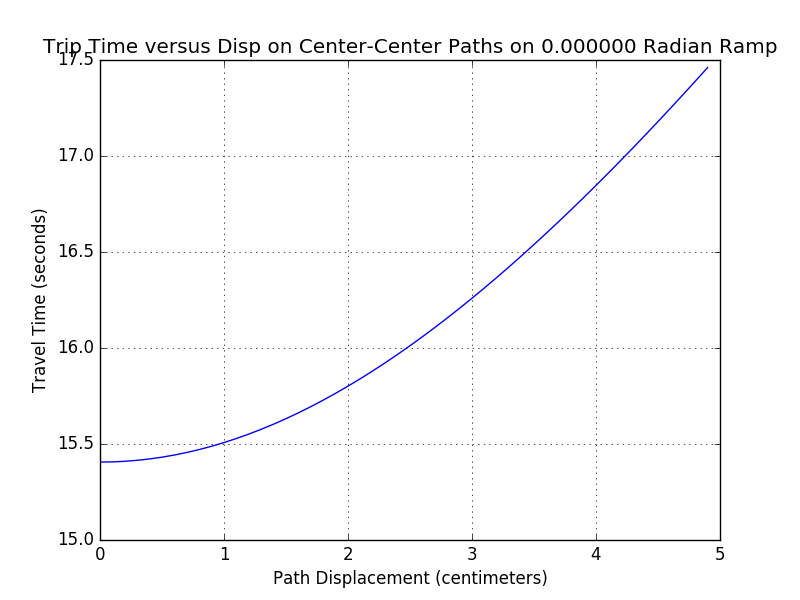
\includegraphics[width=0.2\textwidth]{img/center_center_trip_time_vs_displacement_0_radian_ramp}%
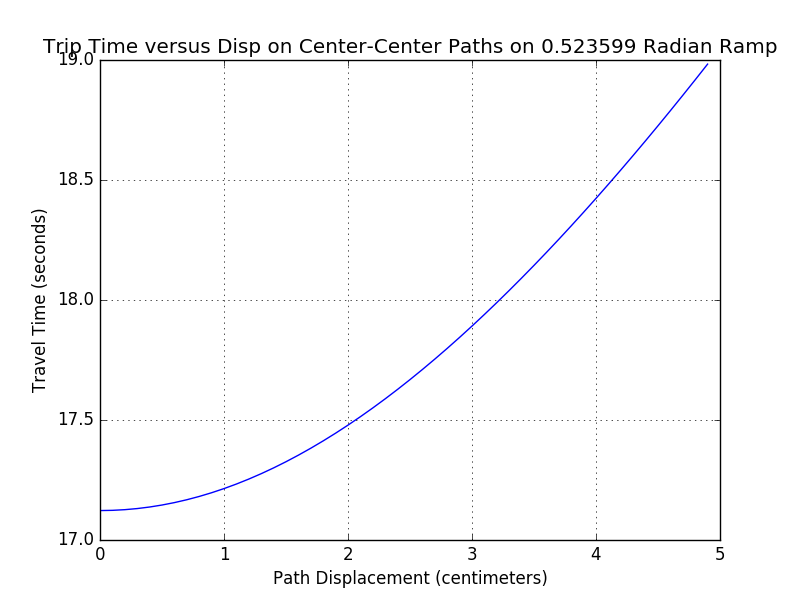
\includegraphics[width=0.2\textwidth]{img/center_center_trip_time_vs_displacement_pi_6_radian_ramp}%
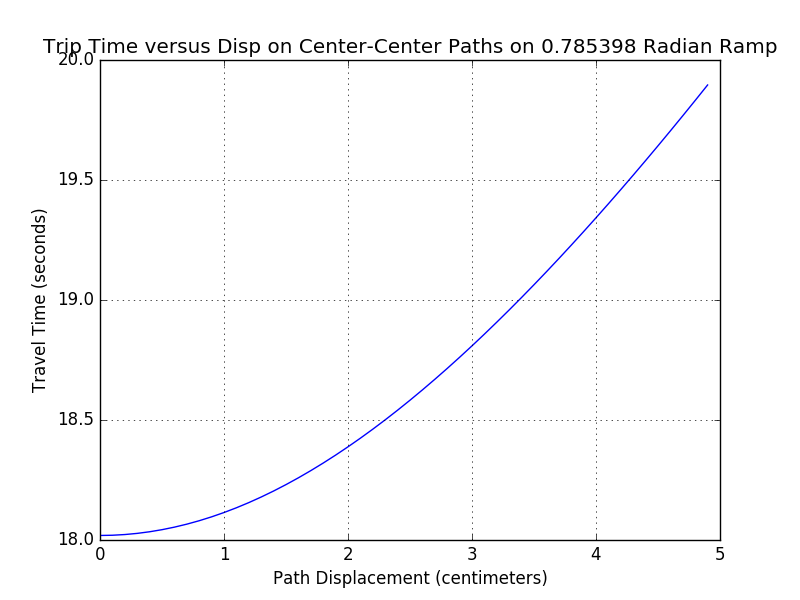
\includegraphics[width=0.2\textwidth]{img/center_center_trip_time_vs_displacement_pi_4_radian_ramp}%
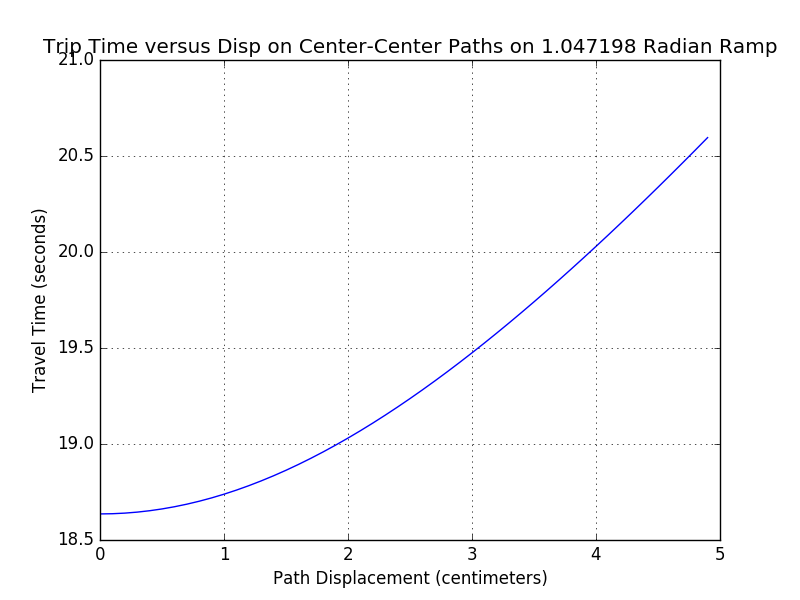
\includegraphics[width=0.2\textwidth]{img/center_center_trip_time_vs_displacement_pi_3_radian_ramp}%
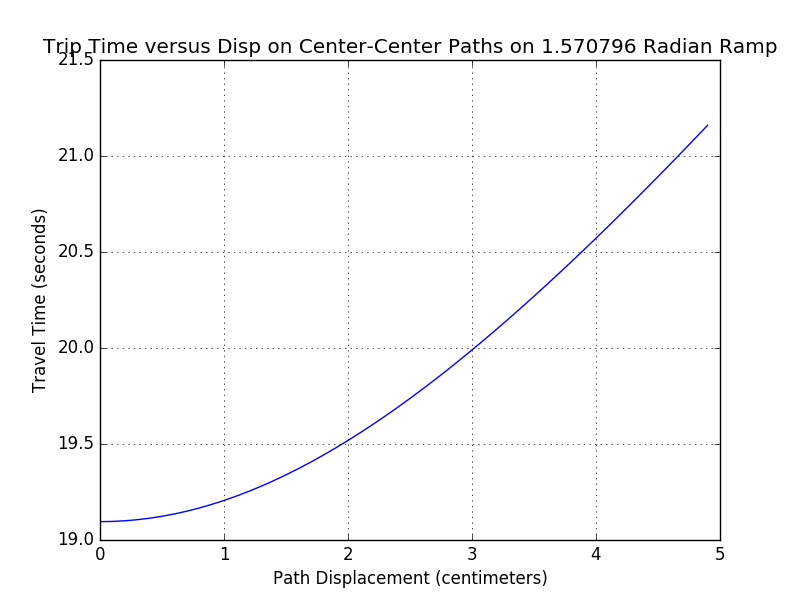
\includegraphics[width=0.2\textwidth]{img/center_center_trip_time_vs_displacement_pi_2_radian_ramp}%
\begin{center}
\begin{tabular}{ c c c }
 incline & displacement (cm) & time (sec) \\ 
 0 & -1.7974794563099371e-07 & 15.405786655568573 \\  
 math.pi/6 & 5.6617903973553256e-07 & 17.122658476770816 \\
 math.pi/4 & 1.0261720572201424e-06 & 18.01885399004196 \\
 math.pi/3 & 5.9487996206179609e-07 & 18.635815540816168 \\
 math.pi/2 & 1.1626086887780648e-06 & 19.09558878811987
\end{tabular} \\
displacement for a direct path: 0
\end{center}


\input{fig/optimalpath_centercenter.tex}

\input{fig/optimalpath_cornercorner.tex}

\bibliography{sample}
\bibliographystyle{apalike}

\end{document}